\documentclass[12pt]{article}

% Paquetes necesarios
\usepackage[utf8]{inputenc}
\usepackage[T1]{fontenc}
\usepackage[spanish]{babel}
\usepackage{graphicx}
\usepackage{geometry}
\usepackage{titling}
\usepackage{setspace}
\usepackage{fancyhdr}
\usepackage{amsmath}


% Márgenes
\geometry{left=3cm, right=3cm, top=3cm, bottom=3cm}

% No hay número de página en la portada
\pagestyle{empty}

\begin{document}

% ------------------------ PORTADA ------------------------
\begin{titlepage}
    \begin{center}
        
        {\Huge\bfseries Aproximación por Mínimos Cuadrados}
        \vspace*{2cm}

        
        \includegraphics[width=0.4\textwidth]{"paleta.jpeg"}
        
        \vspace*{4cm}
        
        
        \begin{flushleft}
            {\large\textbf{Materia:} Análisis Numérico}\\[0.5cm]

            {\large\textbf{Comisión:} K3053}\\[0.5cm]

            {\large\textbf{Integrante:} Erik Flores} \\[0.5cm]

            {\large\textbf{Fecha:} 7 de julio de 2025}\\
        \end{flushleft}
        
        \vfill
        
    \end{center}
\end{titlepage}

% ------------------------ CONTENIDO ------------------------
\newpage
\pagestyle{plain}  
    \newpage
    \section*{Descripción general del problema }

    El presente trabajo práctico tiene como objetivo aplicar el método de mínimos cuadrados para analizar y modelar la relación entre la edad de los jugadores y su puntaje de ranking dentro del sistema oficial de tenis de mesa en Argentina.

    En particular, el estudio se centrará en los jugadores que actualmente compiten en Primera División, una de las categorías más altas del circuito nacional organizado por la plataforma \textit{Tenis de Mesa Para Todos} (TMT). Esta base de datos pública y actualizada brinda información detallada sobre cada jugador federado, incluyendo su edad y el puntaje oficial asignado por el sistema de ranking TMT.

    Dado que el puntaje de ranking varía semanalmente, se ha tomado como referencia la actualización correspondiente al día \textbf{7 de julio de 2025}, para garantizar la coherencia y consistencia de los datos analizados. A partir del listado oficial de 88 jugadores activos en Primera División, se ha seleccionado una muestra representativa de 20 jugadores, procurando abarcar distintas franjas etarias para garantizar diversidad en los datos.

    La intención es construir un modelo matemático que permita estimar qué puntaje de ranking podría alcanzar un jugador en esta categoría en función de su edad, si se mantiene la tendencia observada en los datos actuales.

    Este enfoque no solo permite explorar la dinámica entre edad y rendimiento competitivo en un deporte de alta exigencia como el tenis de mesa, sino también obtener una herramienta predictiva útil, por ejemplo, para entrenadores, jugadores jóvenes o incluso instituciones deportivas que quieran anticipar el potencial competitivo de sus atletas en base a su edad.


    \vspace{1cm}

    % Subtítulo y gráfico
    \subsection*{Nube de puntos}

    \begin{center}
        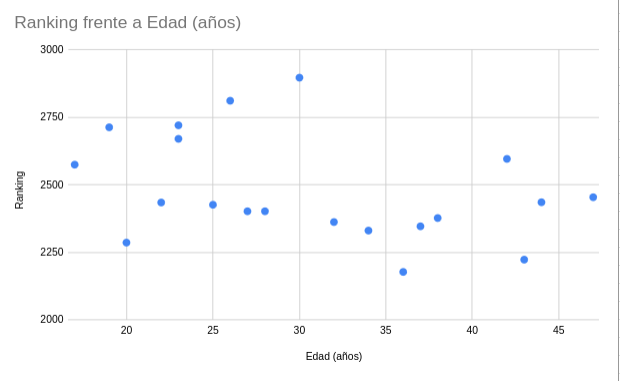
\includegraphics[width=0.75\textwidth]{nube.png}    
    \end{center}


\newpage
\section*{Modelos de Aproximación}

    Con el objetivo de analizar y modelar la relación entre la edad de los jugadores y su puntaje en el ranking, se aplicarán tres enfoques distintos de ajuste de datos: una aproximación lineal, una aproximación exponencial y una aproximación cuadrática.

    Estos modelos permitirán evaluar cuál de ellos se ajusta mejor al comportamiento de los datos observados. Para llevar a cabo este análisis, se trabajará con el siguiente conjunto de datos correspondiente a una muestra de jugadores de Primera División:

    \vspace{1.5cm}

    \begin{center}
        \begin{tabular}{|c|c|}
            \hline
                \textbf{Edad (años)} & \textbf{Ranking} \\
            \hline
            19 & 2714 \\
            17 & 2575 \\
            22 & 2435 \\
            20 & 2287 \\
            26 & 2812 \\
            23 & 2721 \\
            23 & 2671 \\
            25 & 2427 \\
            30 & 2897 \\
            27 & 2403 \\
            28 & 2403 \\
            32 & 2363 \\
            34 & 2331 \\
            37 & 2347 \\
            38 & 2378 \\
            36 & 2178 \\
            44 & 2436 \\
            43 & 2224 \\
            42 & 2597 \\
            47 & 2455 \\
            \hline
        \end{tabular}
    \end{center}

\newpage
    \section*{Aproximación lineal}

        
        Para una función lineal de la forma: $f(x) = a \cdot x + b$


        se construye el sistema de ecuaciones normales utilizando las siguientes expresiones:

        \[
        \left\{
            \begin{array}{l}
                a \cdot \sum\limits_{i=1}^{n} x_i^2 + b \cdot \sum\limits_{i=1}^{n} x_i = \sum\limits_{i=1}^{n} x_i f(x_i) \\
                a \cdot \sum\limits_{i=1}^{n} x_i + b \cdot n = \sum\limits_{i=1}^{n} f(x_i)
            \end{array}
        \right.
        \]



        Donde:

        \begin{itemize}
            \item $x$ representa la edad de cada jugador
            \item $y$ representa el puntaje en el ranking
            \item $n$ es la cantidad total de datos (en este caso, $n = 20$)
        \end{itemize}

\section*{Resolución del sistema por método matricial}

    Tenemos el sistema:

    \[
    \left\{
    \begin{array}{l}
    a \cdot 20353 + b \cdot 613 = 1509285 \\
    a \cdot 613 + b \cdot 20 = 49654
    \end{array}
    \right.
    \]

    \vspace{0.3cm}
    \textbf{Paso 1: Representación matricial}

    \[
    A \cdot X = B
    \]

    Donde:

    \[
    A = 
    \begin{bmatrix}
    20353 & 613 \\
    613 & 20
    \end{bmatrix}, \quad
    X = 
    \begin{bmatrix}
    a \\
    b
    \end{bmatrix}, \quad
    B = 
    \begin{bmatrix}
    1509285 \\
    49654
    \end{bmatrix}
    \]

    \vspace{0.3cm}
    \textbf{Paso 2: Aplicamos la inversa de A}

    \[
    X = A^{-1} \cdot B
    \]

    \vspace{0.3cm}
    \textbf{ Paso 3: Matriz inversa de A}

    \[
    A^{-1} = 
    \begin{bmatrix}
    0.000639 & -0.01959 \\
    -0.01959 & 0.650443
    \end{bmatrix}
    \]

    \vspace{0.3cm}
    \textbf{Paso 4: Multiplicación matricial}

    \[
    X = A^{-1} \cdot B = 
    \begin{bmatrix}
    0.000639 & -0.01959 \\
    -0.01959 & 0.650443
    \end{bmatrix}
    \cdot
    \begin{bmatrix}
    1509285 \\
    49654
    \end{bmatrix}
    =
    \begin{bmatrix}
    -8.0599 \\
    2729.74
    \end{bmatrix}
    \]

    \vspace{0.3cm}
    \textbf{Función aproximante final}

    \[
    f(x) = -8.06 \cdot x + 2729.74
    \]\vspace{1cm}

    A continuación, se presenta la tabla con los cálculos necesarios que se usaron para resolver el sistema de ecuaciones.

        \vspace{0.5cm}
        \begin{center}
            \renewcommand{\arraystretch}{1.3}
            \begin{tabular}{|c|c|c|c|}
                \hline
                \textbf{Edad (x)} & \textbf{Ranking (y)} & $x^2$ & $x \cdot y$ \\
                \hline
                19 & 2714 & 361 & 51566 \\
                17 & 2575 & 289 & 43775 \\
                22 & 2435 & 484 & 53570 \\
                20 & 2287 & 400 & 45740 \\
                26 & 2812 & 676 & 73112 \\
                23 & 2721 & 529 & 62583 \\
                23 & 2671 & 529 & 61433 \\
                25 & 2427 & 625 & 60675 \\
                30 & 2897 & 900 & 86910 \\
                27 & 2403 & 729 & 64881 \\
                28 & 2403 & 784 & 67284 \\
                32 & 2363 & 1024 & 75616 \\
                34 & 2331 & 1156 & 79254 \\
                37 & 2347 & 1369 & 86839 \\
                38 & 2378 & 1444 & 90364 \\
                36 & 2178 & 1296 & 78408 \\
                44 & 2436 & 1936 & 107184 \\
                43 & 2224 & 1849 & 95632 \\
                42 & 2597 & 1764 & 109074 \\
                47 & 2455 & 2209 & 115385 \\
                \hline
                    \textbf{$\sum x = 613$} & \textbf{$\sum y = 49654$} & \textbf{$\sum x^2 = 20353$} & \textbf{$\sum xy = 1509285$} \\
                \hline
            \end{tabular}
        \end{center}

        \vspace{0.5cm}

\vspace{1cm}


    \vspace{1cm}
        Ahora se presenta el gráfico de la recta obtenida superpuesta sobre la nube de puntos original, lo cual permite visualizar el ajuste lineal al conjunto de datos:

    \vspace{0.5cm}

    \begin{center}
        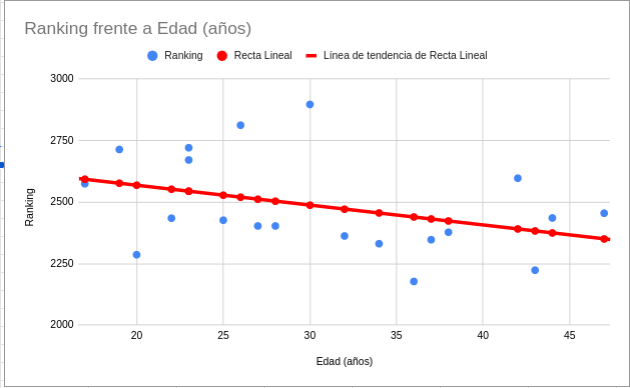
\includegraphics[width=0.75\textwidth]{rectaNubeDePuntos.png}
    \end{center}






%exponencial

\section*{Modelo exponencial}

Queremos ajustar un modelo del tipo:

\[
f(x) = b \cdot e^{a \cdot x}
\]

Aplicando logaritmo natural a ambos lados:

\[
\ln(y) = \ln(b) + a \cdot x
\]

Definimos:

\[
Y = \ln(y), \quad A = a, \quad B = \ln(b)
\]

Entonces, el modelo queda linealizado:

\[
Y = A \cdot x + B
\]

\vspace{0.5cm}
\textbf{ Paso 1: Cálculo de valores transformados}

A continuación, se presenta la tabla con los valores de \( x \), \( y \), \( \ln(y) \), \( x \cdot \ln(y) \) y \( x^2 \), utilizados para la estimación por mínimos cuadrados:

\vspace{0.3cm}

\begin{center}
\renewcommand{\arraystretch}{1.2}
\begin{tabular}{|c|c|c|c|c|}
\hline
\textbf{Edad (x)} & \textbf{Ranking (y)} & \textbf{ln(y)} & \textbf{x·ln(y)} & \textbf{x²} \\
\hline
19 & 2714 & 7.9062 & 150.2174 & 361 \\
17 & 2575 & 7.8536 & 133.5113 & 289 \\
22 & 2435 & 7.7977 & 171.5494 & 484 \\
20 & 2287 & 7.7350 & 154.6999 & 400 \\
26 & 2812 & 7.9417 & 206.4829 & 676 \\
23 & 2721 & 7.9088 & 181.9014 & 529 \\
23 & 2671 & 7.8902 & 181.4748 & 529 \\
25 & 2427 & 7.7944 & 194.8603 & 625 \\
30 & 2897 & 7.9714 & 239.1429 & 900 \\
27 & 2403 & 7.7845 & 210.1808 & 729 \\
28 & 2403 & 7.7845 & 217.9653 & 784 \\
32 & 2363 & 7.7677 & 248.5660 & 1024 \\
34 & 2331 & 7.7541 & 263.6378 & 1156 \\
37 & 2347 & 7.7609 & 287.1530 & 1369 \\
38 & 2378 & 7.7740 & 295.4126 & 1444 \\
36 & 2178 & 7.6862 & 276.7018 & 1296 \\
44 & 2436 & 7.7981 & 343.1170 & 1936 \\
43 & 2224 & 7.7071 & 331.4037 & 1849 \\
42 & 2597 & 7.8621 & 330.2087 & 1764 \\
47 & 2455 & 7.8059 & 366.8765 & 2209 \\
\hline
\textbf{613} & \textbf{49654} & \textbf{156.2839} & \textbf{4785.0634} & \textbf{20353} \\
\hline
\end{tabular}
\end{center}

\vspace{1cm}
\section*{Resolvemos el sistema de ecuación Lineal}


Reemplazando con los valores obtenidos:

\[
\left\{
\begin{array}{l}
a \cdot 20353 + b \cdot 613 = 4785.063 \\
a \cdot 613 + b \cdot 20 = 156.284
\end{array}
\right.
\]

\vspace{0.3cm}
\textbf{ Paso 2: Método matricial}

\[
A \cdot X = B
\]

\[
A = 
\begin{bmatrix}
20353 & 613 \\
613 & 20
\end{bmatrix}, \quad
X = 
\begin{bmatrix}
a \\
b
\end{bmatrix}, \quad
B = 
\begin{bmatrix}
4785.063 \\
156.284
\end{bmatrix}
\]

\vspace{0.3cm}
\textbf{ Inversa de A :}

\[
A^{-1} \approx 
\begin{bmatrix}
0.000639 & -0.01959 \\
-0.01959 & 0.65044
\end{bmatrix}
\]

\vspace{0.3cm}
\textbf{ Multiplicación}

\[
X = A^{-1} \cdot B =
\begin{bmatrix}
0.000639 & -0.01959 \\
-0.01959 & 0.65044
\end{bmatrix}
\cdot
\begin{bmatrix}
4785.063 \\
156.284
\end{bmatrix}
\approx
\begin{bmatrix}
-0.00415 \\
7.3538
\end{bmatrix}
\]

\vspace{0.3cm}
\textbf{ Paso 3: Volvemos a la función exponencial}

Sabemos que:

\[
\ln(y) = a \cdot x + \ln(b) \quad \Rightarrow \quad y = b \cdot e^{a \cdot x}
\]

Ya tenemos:

\[
a = -0.00415, \quad \ln(b) = 7.3538 \quad \Rightarrow \quad b = e^{7.3538} \approx 1563.82
\]

\vspace{0.3cm}
\textbf{Función aproximante final (modelo exponencial):}

\[
f(x) = 1563.82 \cdot e^{-0.00415 \cdot x}
\]

\vspace{1cm}
\subsection*{Visualización del modelo exponencial ajustado}

\vspace{0.5cm}

\begin{center}
    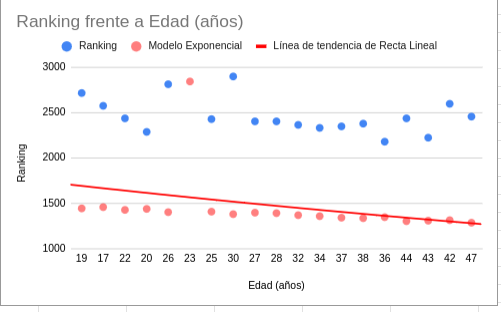
\includegraphics[width=0.75\textwidth]{nubeExponencial.png}
\end{center}


\end{document}
